\documentclass[11pt]{article}

%%%%%%%%%%%%%%Include Packages%%%%%%%%%%%%%%%%%%%%%%%%%%
\usepackage{xcolor}
\usepackage{mathtools}
\usepackage[a4paper, total={6in, 8in}, margin=1.25in]{geometry}
\usepackage{amsmath}
\usepackage{amssymb}
\usepackage{paralist}
\usepackage{rsfso}
\usepackage{amsthm}
\usepackage{wasysym}
\usepackage[inline]{enumitem}   
\usepackage{hyperref}
\usepackage{tocloft}
\usepackage{titlesec}
\usepackage{colortbl}
\usepackage{wrapfig}
\usepackage{pdfpages}
%%%%%%%%%%%%%%%%%%%%%%%%%%%%%%%%%%%%%%%%%%%%%%%%%%%%%%%%



\begin{document}
\Large \noindent \textbf{Physics 5A Discussion (Week 2)}\\
\normalsize
Department of Physics and Astronomy, UCLA\\
\noindent\rule{8cm}{0.4pt}\\


\begin{center}
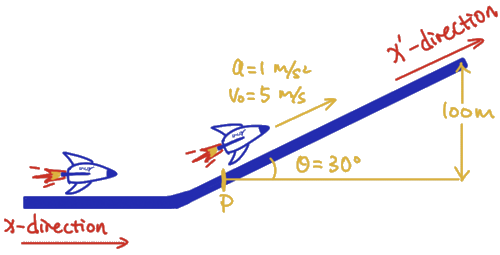
\includegraphics[scale=0.5]{rocket2}
\end{center}
\noindent \textbf{Problem 1}: After accelerating to the right for a few seconds, the rocket moves onto a ramp at an angle of $\theta = 30^\circ$. When it reaches point $P$ as shown, it has an instantaneous velocity $v_0 = 5$ m/s in the $x'$-direction, and its acceleration in the $x'$-direction is kept constant at $1$ m/s$^2$. How long does it take for the rocket to reach a height of $h = 100 $ m? This is quite a complicated problem, but we can break it down into a few steps:\\

\textbf{Step 1:} Looking at the triangle shown, how far does the rocket need to travel in the $x'$-direction (distance on the ramp) to reach $h=100$ m?
\newline\newline\newline\newline


\textbf{Step 2:} Draw the acceleration vs.\ time graph, with the acceleration in the $x'$-direction on the vertical axis, and time on the horizontal axis. \textit{(Hint: As mentioned in the problem, acceleration is kept constant over time.)}\\
\newline\newline\newline
\newline\newline

\textbf{Step 3:} Using the graph you have in step 2, draw the velocity vs.\ time graph for the first $20$ seconds. (\textit{Hint: Change in velocity is the ``area" under the acceleration curve.})\\
\newline\newline\newline
\newline\newline

\textbf{Step 4:} Using the graph you have in step 3, what is the shape of curve in your position vs. time graph? (Hint: The slope of your position curve at each time instant should be the value of your velocity curve at the same time instant. Alternatively, the change in the area under the velocity curve corresponds to the amount of increase/decrease in the position curve.)


\textbf{Step 5:} Again using your velocity vs. time graph, how far has the rocket traveled in the $x'$-direction in the first $20$ seconds? (\textit{Hint: Use the "area" under the velocity curve to find displacement.})
\newline\newline\newline
\newline\newline\newline

\textbf{Step 6:} Recall the distance calculated in step 1, how long does the rocket take to travel such a distance? (\textit{Hint: Try an arbitrary final time $t_{\text{f}}$ and repeat from step 3. You will need the quadratic formula when computing your final answer.})
\newline\newline\newline
\newline\newline\newline

\textbf{Step 7:} Now you have seen that \textit{position curve looks like a parabola if we have a constant acceleration over time}, this result leads to the kinematic equation that you will see very soon during lecture:
\begin{align*}
x = \frac{1}{2}at^2 + v_0 t + x_0\,,
\end{align*}
where $x_0$ is your initial position at time $t = 0$ second, and $x$ is your final position at a generic time $t$. Using this formula, find the time $t$ for the rocket to travel from $x_0 = 0$\,m  to $x = \,$(your result in step 1) in the $x'$-direction. (\textit{Hint: You will need the quadratic formula. The result you get here should agree with the one you found in step 6.})
\newline\newline\newline
\newline\newline\newline
\newline\newline\newline


\noindent \textbf{Problem 2}: For the rocket in problem 1, how far has the rocket traveled in the horizontal direction ($x$-direction) when it reaches $h = 100$ m?
\newline\newline\newline
\newline\newline\newline
\newline\newline\newline
Review the week-1 worksheet (rocket moving left and right) if you have time :)\\
Especially if you want some practice on ``average speed" and ``average velocity". 

\includepdf[pages=-]{w2}

\end{document}


